\subsection{Program Structure}
As mentioned \todo{before or above missing?}{Morten} our server is written in F\Sh which is a very powerful functional programming language with pattern matching and parallel programming abilities.
F\Sh can even be object oriented, but we have chosen to stick with the functional paradigm: We wanted the exercise of writing a purely functional system.

Our system is built of modules which are put together like bricks into layers that form a great structure. \todo{Not quite satisfied with this formulation}{Michael}
\\We have an Outer Layer - or shell - which is the published web services. This layer is actually written in C\Sh using the Windows Communications Foundation.
\\Then we have a Security Layer which uses a Permission Module to verify users and permissions before invoking functions deeper.
\\The Application Logic Layer is the actual working layer which has Account Module, Product Module and more.
\\The Persistence Layer is the lowest logic layer \todo{This sounds to me like the persistence layer is stupid and/or of poor character}{Morten}. It has the responsibility to create, save and update information on some sort of data storage.
\\Finally we have our Database in which we store our data.

Each Module can be replaced and the Checking Layer is entirely optional. For example one might want to change the Persistence Layer to persist against a file-system instead of a database, or one might want to do less or more extensive checks in the Checking Layer, without changing any of the other layers.

\subsubsubsection{Outer Layer}
We planned to write a thin C\Sh layer. The only responsibility for this layer would be to call the corresponding F\Sh functions. This, however, did not go as planned.

The layer ended up being responsible for receiving data, converting data and sending this to the F\Sh function. When data were to be extracted the layer was responsible for receiving data from F\Sh, converting data and sending it to the client.

This actually turned out to be okay, as we, in theory, could create a SOAP web service without any hassle, and we could possible extend it to different other services as well.

\subsubsubsection{Security Layer}\todo{Consistency...}{Michael}
Our security layer is responsible for checking that the invoking user has the permission required to perform the request. It could possibly do more than just check permissions.

We have created this layer, so that it can be removed without losing any functionality.
\subsubsubsection{Application Logic Layer}
In this layer we perform all our application logic. It is completely unaware of how data is stored however. Data selection and storage is handled elsewhere.
\subsubsubsection{Persistence Layer}
This layer is responsible for storing data. It has been made as generic as possible, so if we chose to change storage to \todo{a file? or?}{k} file instead it would be easy. It is also possible to easily implement a separate search-server if needed.

\begin{figure}[H]
  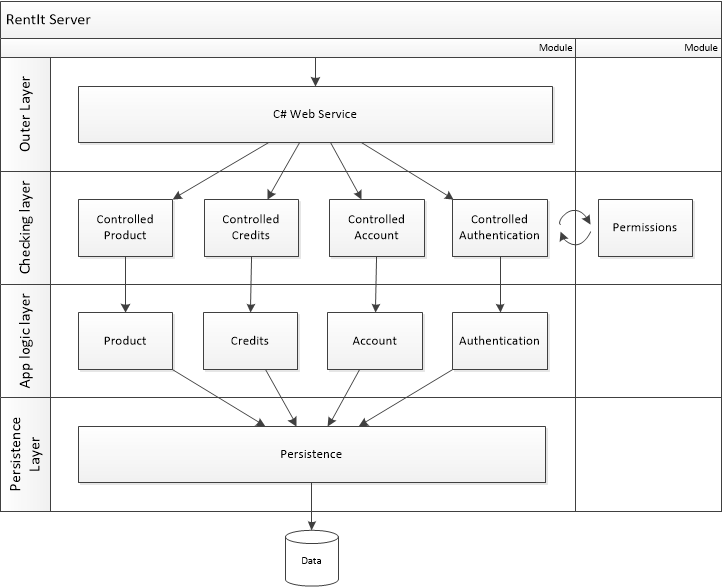
\includegraphics[width=\textwidth]{illustrations/ServerStructure.png}
  \caption{Our Server Structure}
  \label{fig:serverstructure}
\end{figure}
\newpage